\subsubsection{アーキテクチャについての推論}
アーキテクチャ評価は、明確なアーキテクチャ記述があるほど効果的である。ビュー、モデル、意思決定記録があれば、それらを調べ、質問し、分析できる。信頼性、安全性、セキュリティのような専門的関心事では、それぞれの分野で使われる専門的な表現が必要になることがある。

しかし、現実にはアーキテクチャ文書が未完成、不完全、古い、存在しない場合も多い。その場合、評価は関係者の知識に依存する。これは危険である。なぜなら、人の記憶は抜け落ちやすく、関係者が退職すると知識も失われるからである。

ユースケースは、アーキテクチャの完全性と整合性を確認する手段として使える。ユースケースの各ステップを見て、そのステップを実現する構成要素がアーキテクチャに存在するか、必要な通信やデータが説明されているかを確認する。

\begin{figure}[htbp]
\centering
\IfFileExists{swebok_structure/CH02.ソフトウェアアーキテクチャ(Software_Architecture)/2.4.ソフトウェアアーキテクチャ評価(Software_Architecture_Evaluation)/2.4.2.アーキテクチャについての推論(Reasoning_about_Architectures)/assets/fig-ch02-08.png}{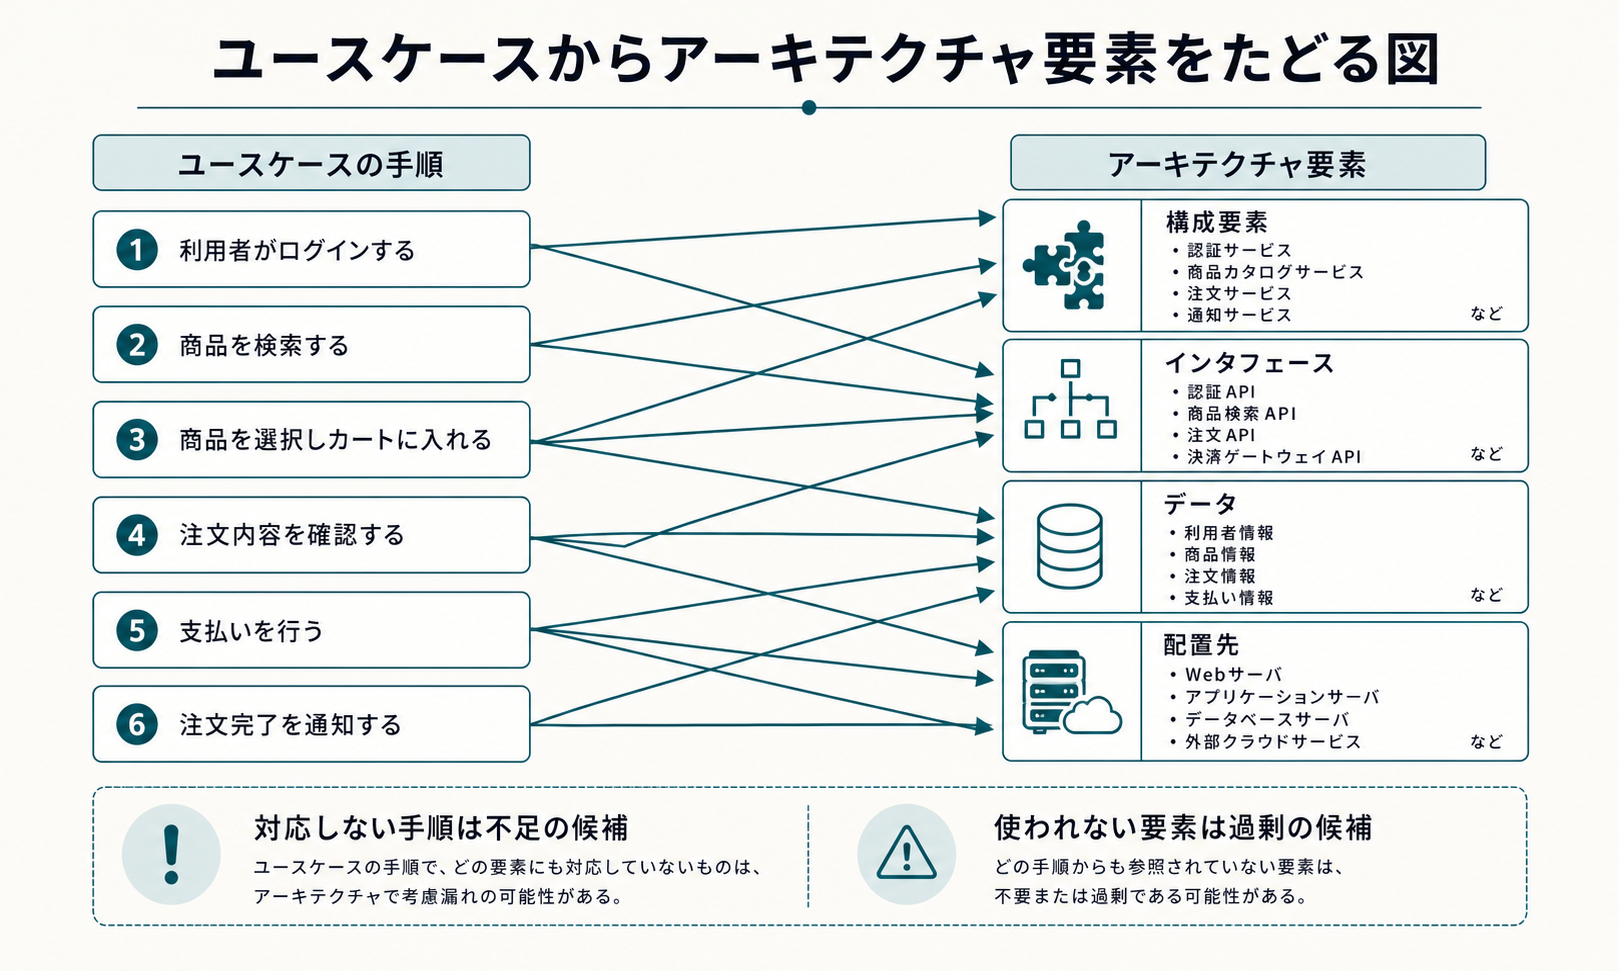
\includegraphics[width=0.96\linewidth]{swebok_structure/CH02.ソフトウェアアーキテクチャ(Software_Architecture)/2.4.ソフトウェアアーキテクチャ評価(Software_Architecture_Evaluation)/2.4.2.アーキテクチャについての推論(Reasoning_about_Architectures)/assets/fig-ch02-08.png}}{\fbox{\parbox[c][48mm][c]{0.9\linewidth}{\centering 画像生成待ち\\ユースケースからアーキテクチャ要素をたどる図}}}
\caption{ユースケースからアーキテクチャ要素をたどる図}
\label{fig:ch02-08}
\end{figure}
